%
%==> Section 3: Remote repositories
%
\section{
  Remote repositories
}

%
%==> Main competitors
%
\begin{frame}
  \frametitle{
    Remote repositories - Main competitors
  }

  \begin{itemize}%[<+->]
  \item
    GitHub: \href{https://github.com/}{https://github.com/}
  \item
    Bitbucket: \href{https://bitbucket.org/}{https://bitbucket.org/}
  \end{itemize}
\end{frame}

%
%==>  Create your own remote repository
%
\begin{frame}[fragile]
  \frametitle{
    Create your own remote repository
  }

  Create your own repository on \textcolor{red}{GitHub (\$7 a month for private repo's)} or \textcolor{blue}{Bitbucket (free unlimited private repo's)}.

  \bigskip  

  This can be for an existing or a new project.

  \bigskip
  
  {\bf More commands:}
  \begin{itemize}
  \item
    {\tt git clone} - imports a remote repository.
  \item
    {\tt git pull} - extracts most recent changes from a repository.
  \item
    {\tt git push} - broadcast your changes to a repository.
  \end{itemize}

\end{frame}

%
%==>  A distant repository with GitHub
%
\begin{frame}[fragile]
  \frametitle{
    A distant repository with GitHub
  }

  % Remark: Up to now, we've been working locally on our computer. As a scientist, you may want to share your work, (or better contribute to an opensource project!). This is where Bitbucket comes in handy. Bitbucket is a web hosting platform for git projects. Not only does it provide free git repository for opensource projects (private repo's are free for up to 5 group users), but it provides great tools to review code, manage projects, release packages and publish documentation.
  
% Now, let's go on Bitbucket, and create an account. Once this is done, We can easily create a new project by clicking on the create button, on the main page.

  \begin{center}
    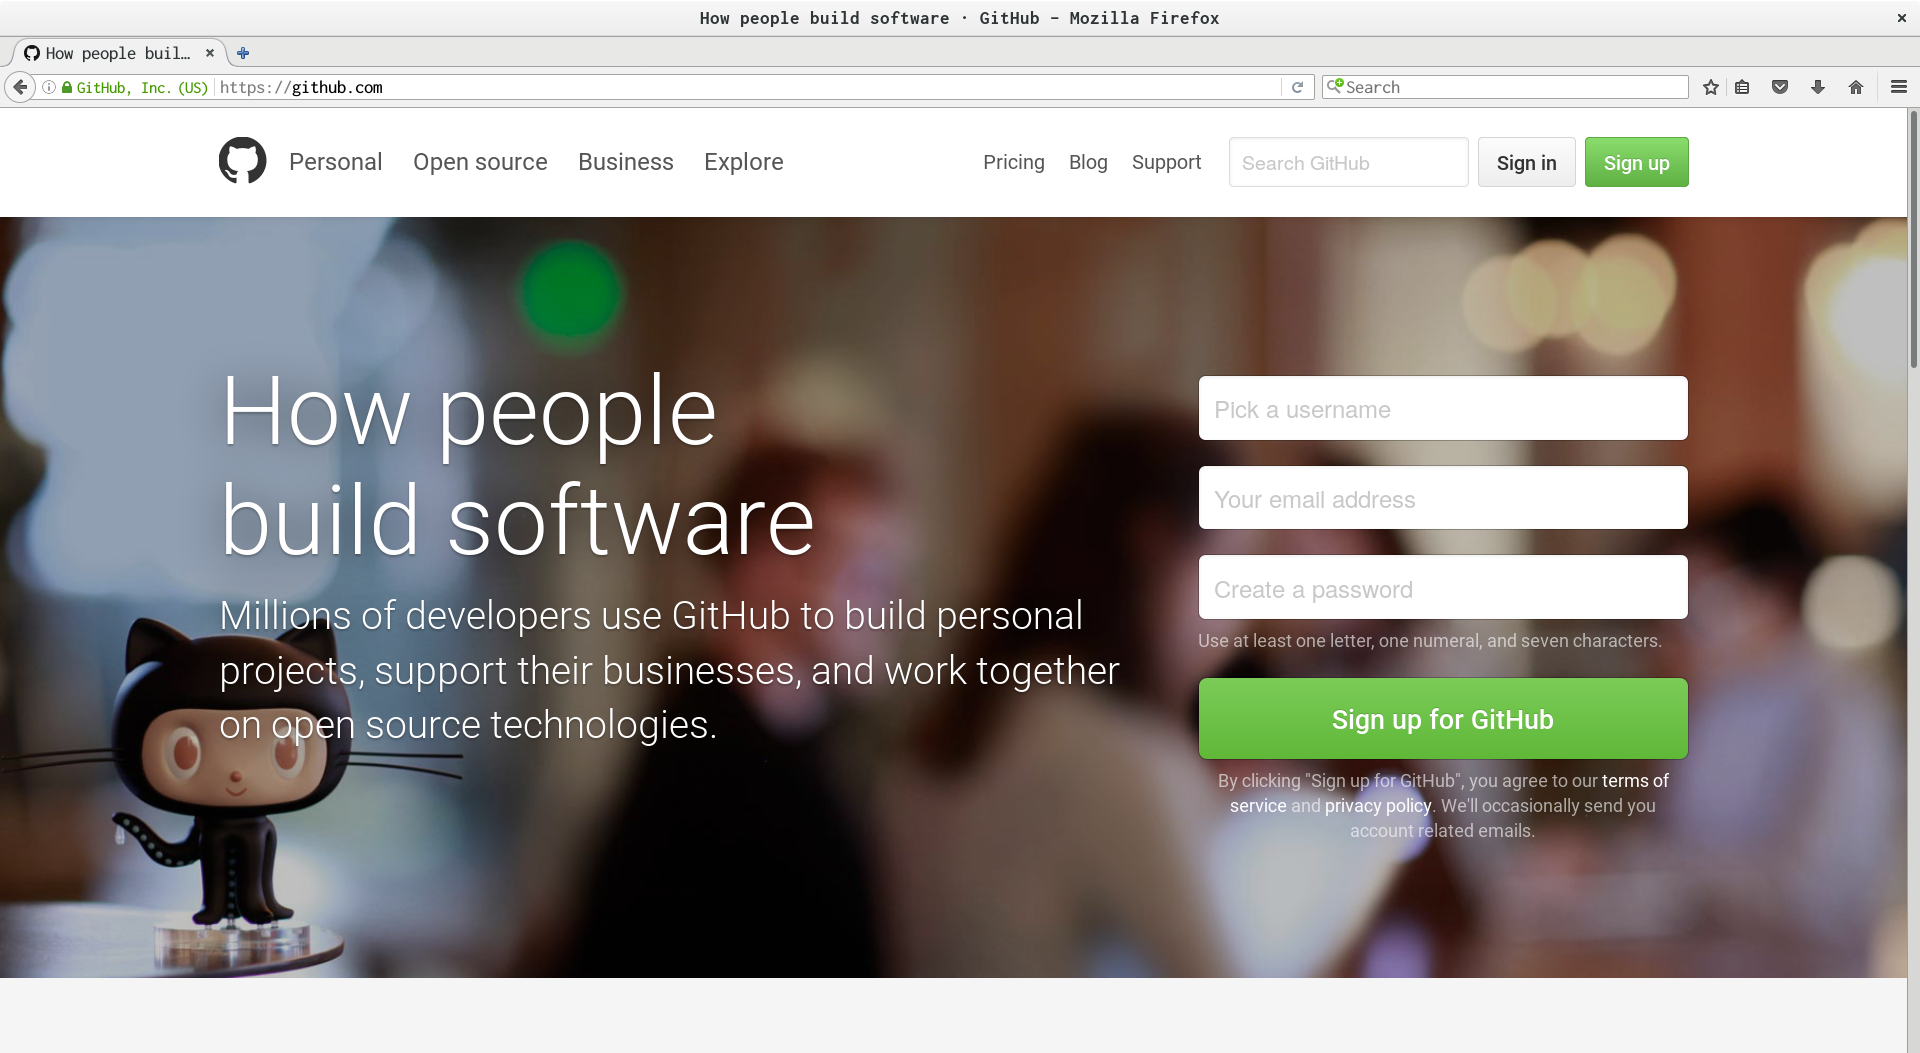
\includegraphics[scale=0.155]{./graphics/github_homepage.png}
  \end{center}

\end{frame}
%
%==> GitHub profile
%
\begin{frame}[fragile]
  \frametitle{
   GitHub profile
  }

  \begin{center}
    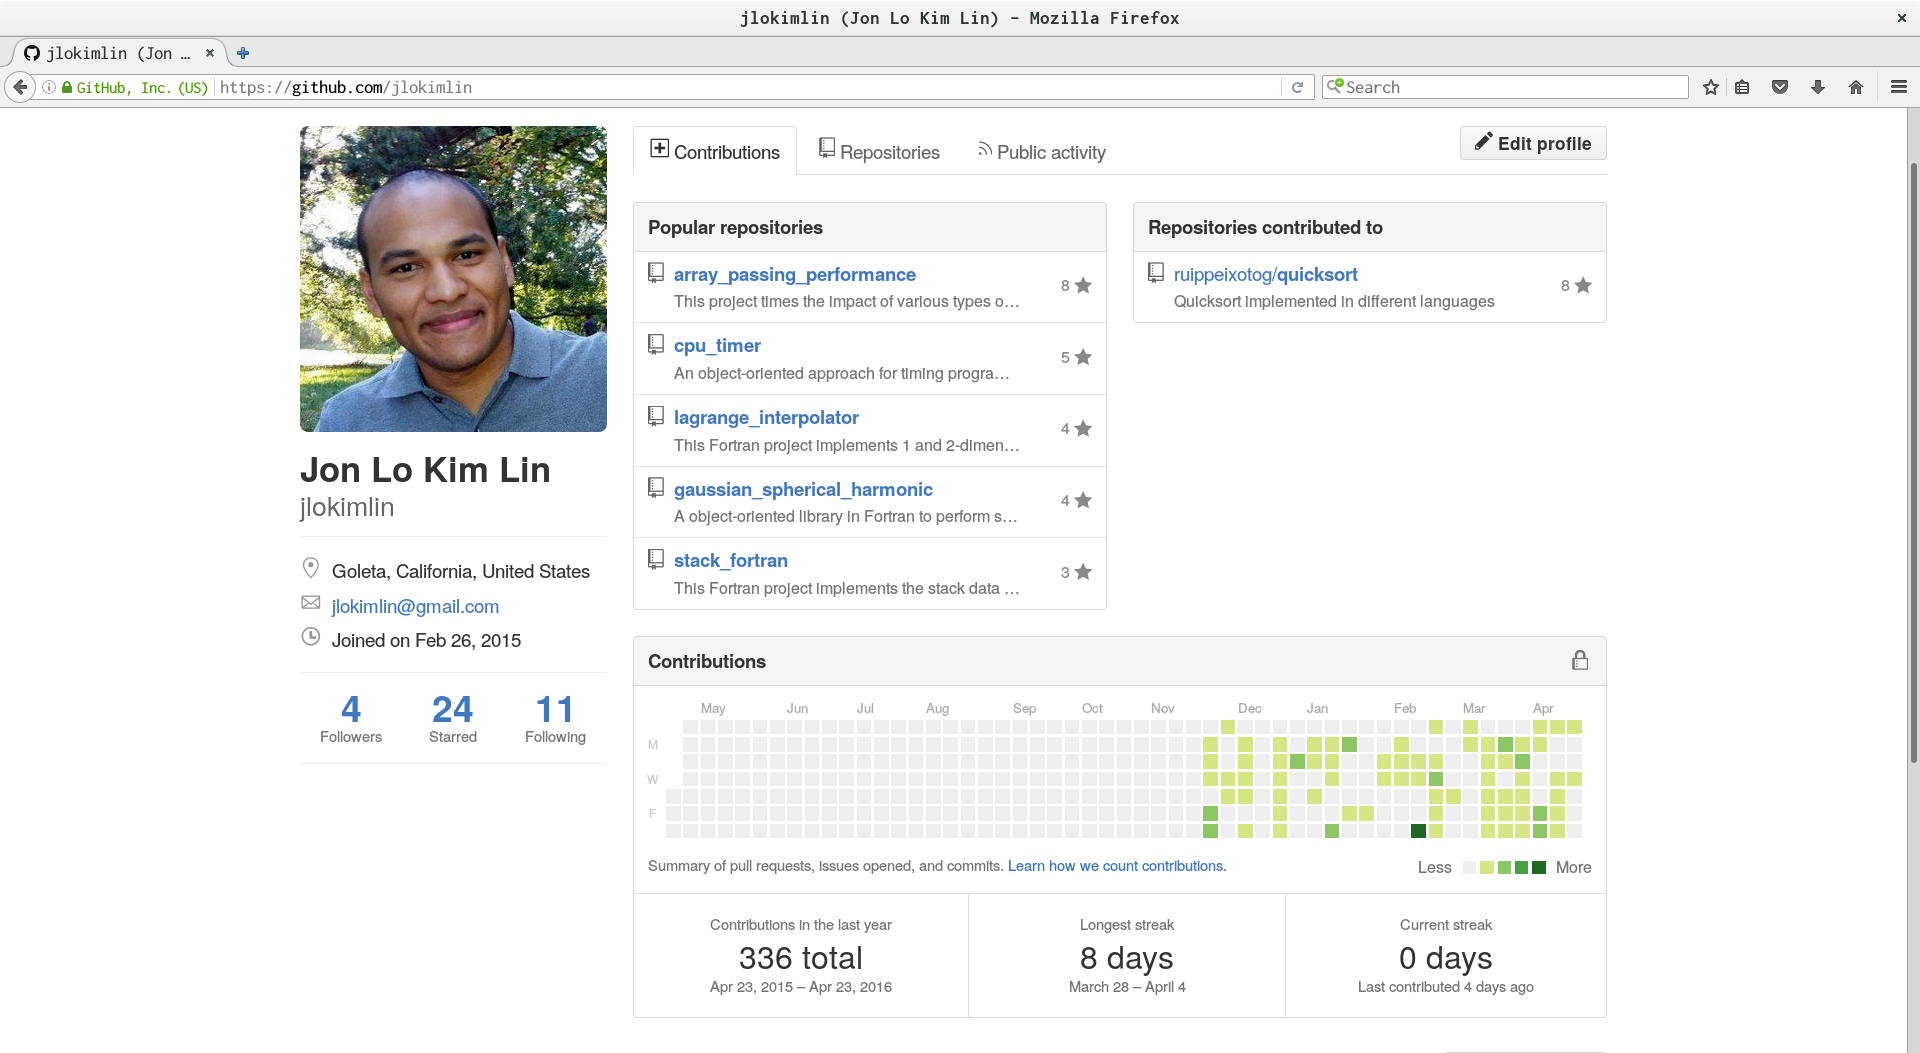
\includegraphics[scale=0.155]{./graphics/jlokimlin_github_profile.png}
  \end{center}

\end{frame}
%
%==> Create new repository
%
\begin{frame}[fragile]
  \frametitle{
    Create new repository
  }

  \begin{center}
    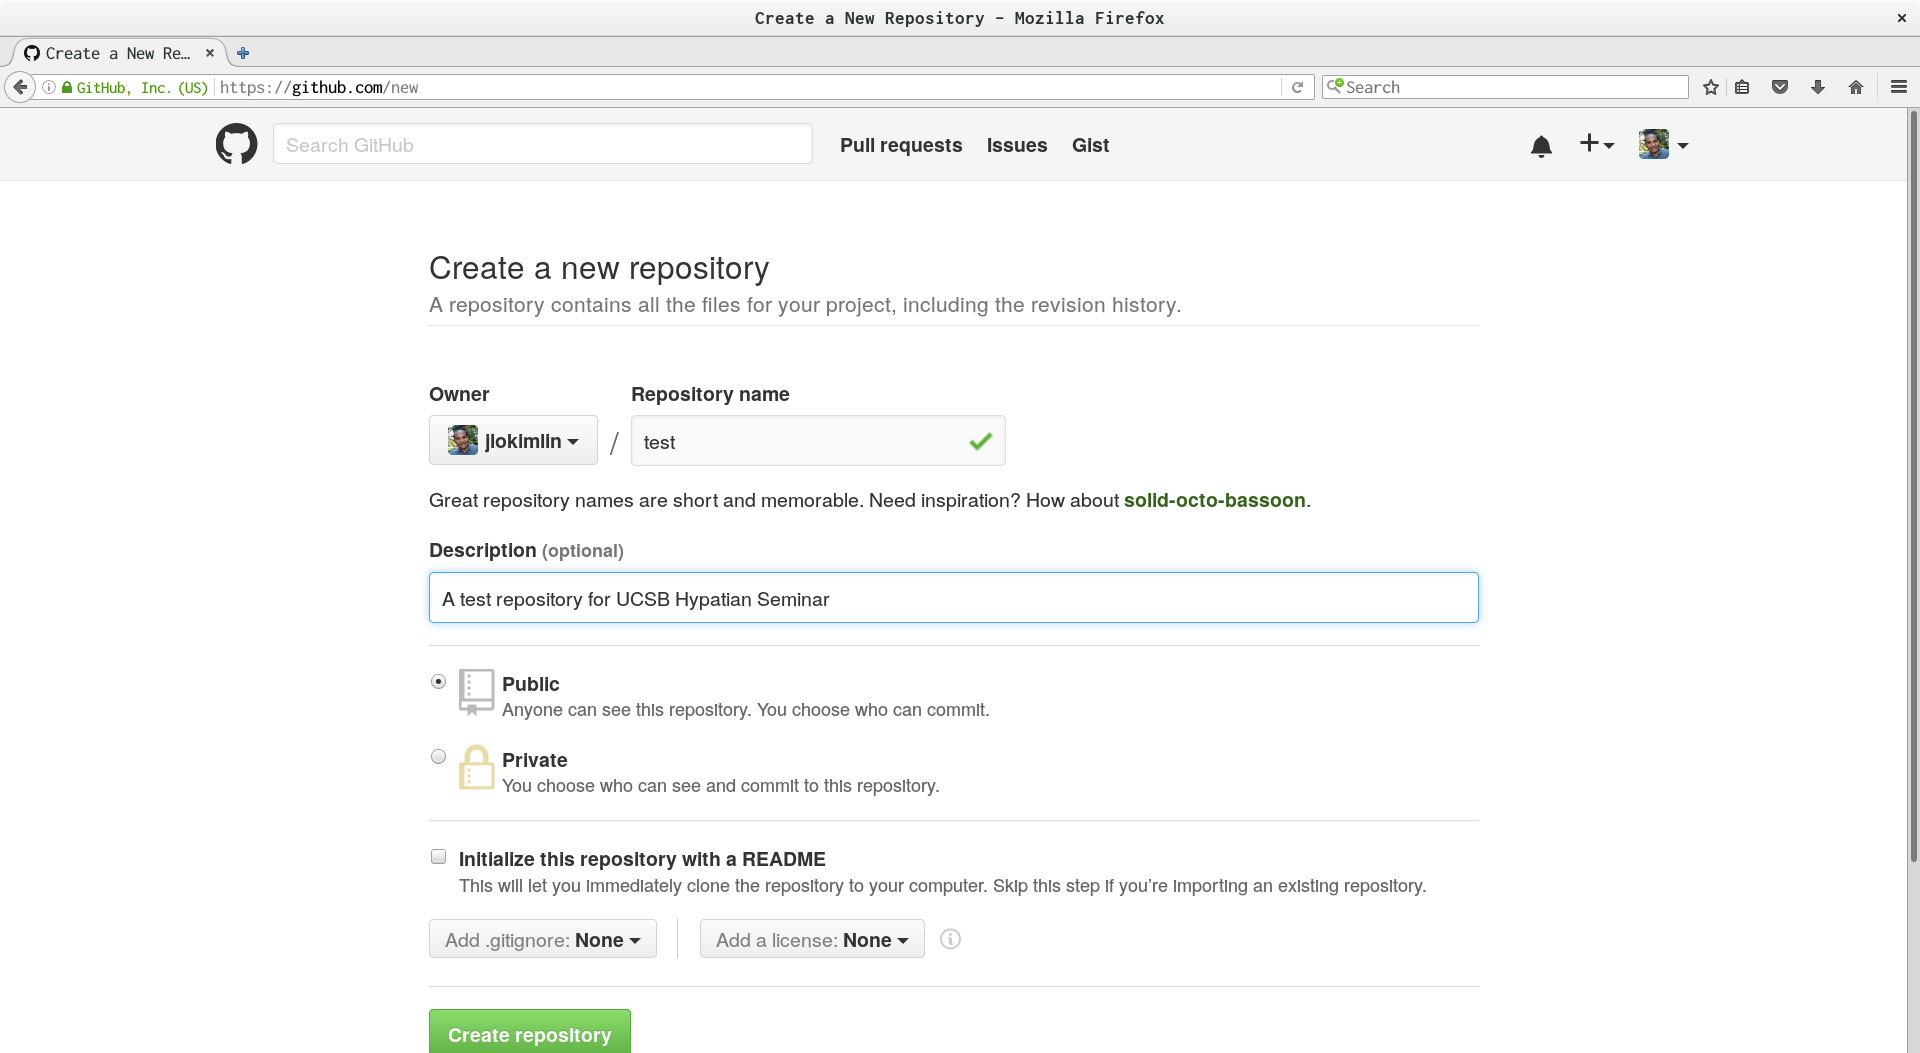
\includegraphics[scale=0.155]{./graphics/create_new_repository.png}
  \end{center}

\end{frame}

%
%==> A distant repository with Bitbucket (continued)
%
\begin{frame}[fragile]
  \frametitle{
    Create a new repository (continued)
  }
  
  \begin{center}
    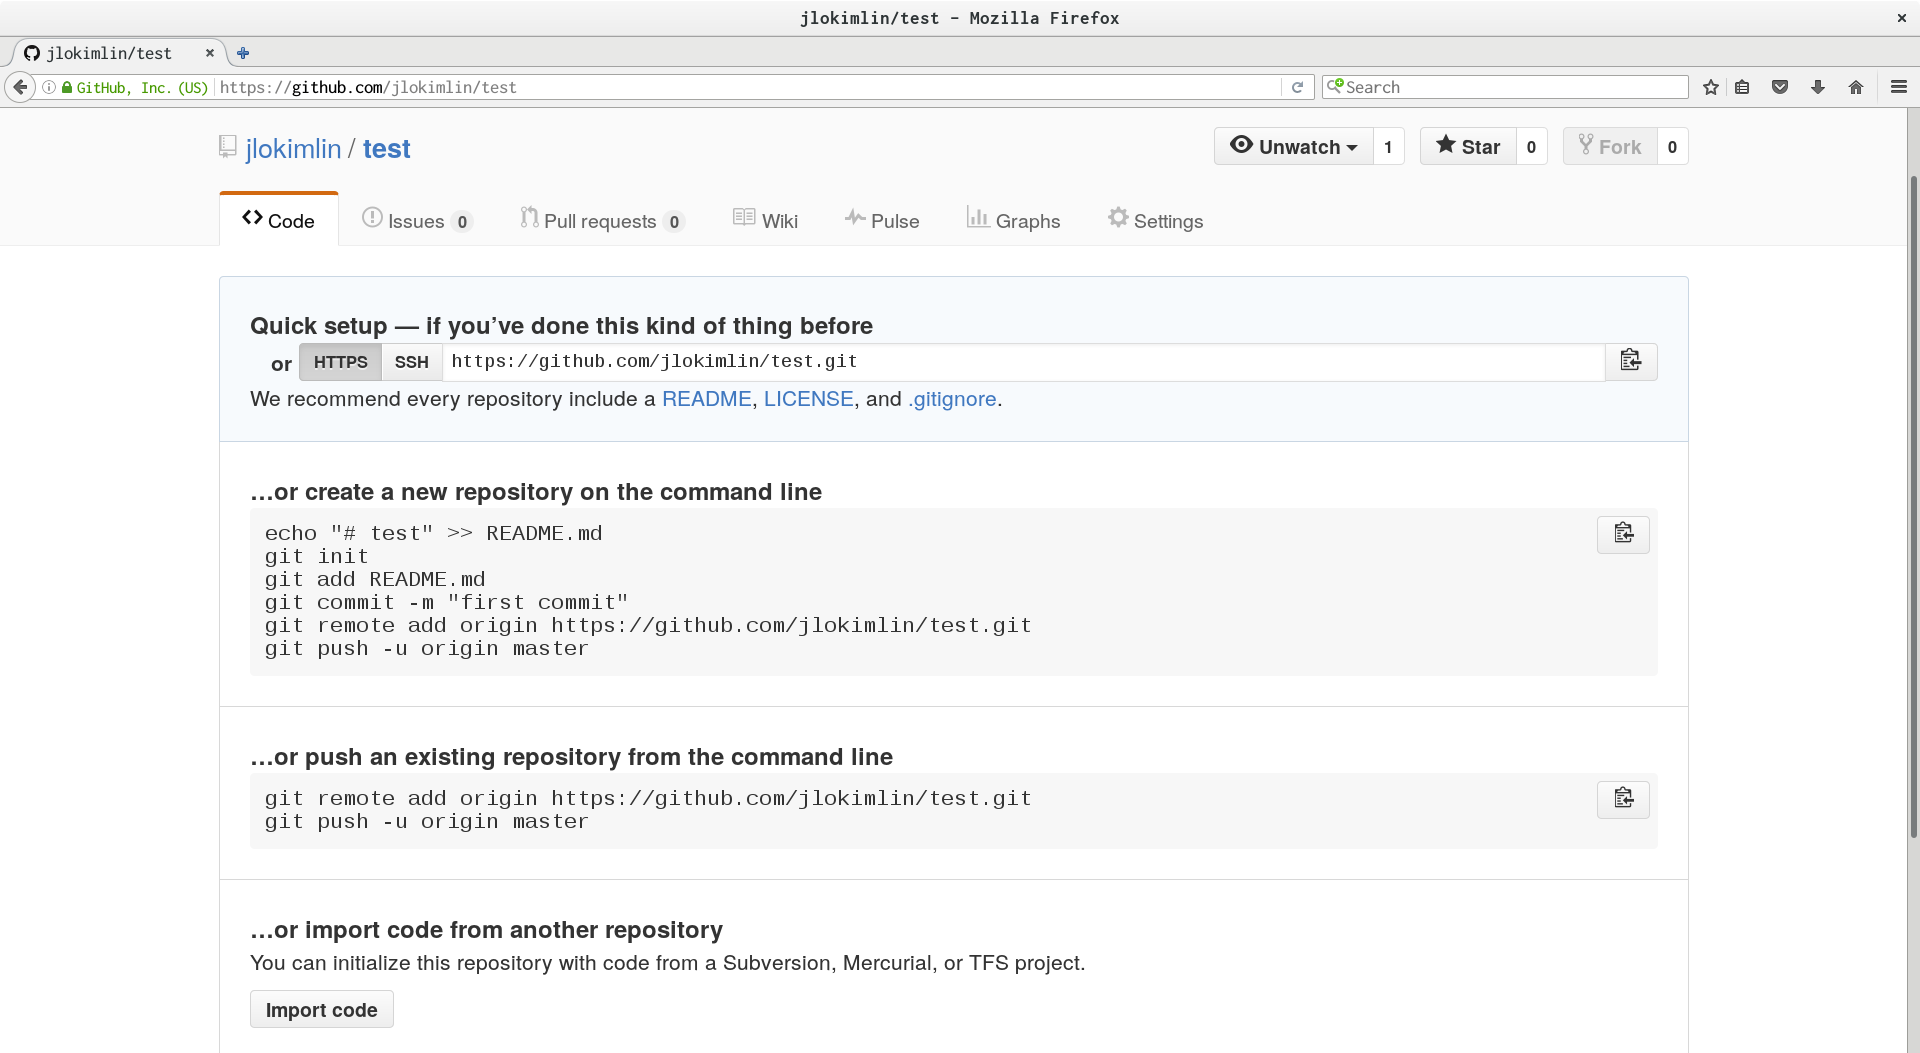
\includegraphics[scale=0.15]{./graphics/new_repo_continued.png}
  \end{center}

\end{frame}

%
%==> Create a new repository on the command line
%
\begin{frame}[fragile]
  \frametitle{
    Create a new repository on the command line
  }

  \begin{lstlisting}
    mkdir /path/to/your/project
    cd /path/to/your/project
    echo "# test" >> README.md
    git init
    git add README.md
    git commit -m "first commit"
    git remote add origin
    https://github.com/jlokimlin/test.git
    git push -u origin master
  \end{lstlisting}
\end{frame}

%
%==> Push an existing repository from the command line
%
\begin{frame}[fragile]
  \frametitle{
    Push an existing repository from the command line
  }

  \begin{lstlisting}
    mkdir /path/to/your/project
    cd /path/to/your/project
    git remote add origin
    https://github.com/jlokimlin/test.git
    git push -u origin master
  \end{lstlisting}

\end{frame}
